%% ============================================================
%%  STANDARD PREAMBLE (article, lecture notes)
%% ============================================================

% ---------- Document class and page layout ----------
\documentclass[11pt]{article}      % Basic document type, 11pt body text
\usepackage[margin=1in]{geometry}  % Sets page margins to 1 inch on all sides

% ---------- Paragraph style ----------
\usepackage{setspace}              % Lets you set the line spacing of the whole document
\setstretch{1.2}                   % Line spacing factor: 1.0 = single (default), 1.2 = slightly airy, 1.5 = very loose
\setlength{\parindent}{2em}        % First-line indent of each paragraph
\setlength{\parskip}{1\baselineskip} % Extra vertical gap between paragraphs

% ---------- Math ----------
\usepackage{amsmath,amssymb}       % Core math: align, cases, \text{}, plus extra symbols (\mathbb, \hbar, ...)

% ---------- Colors and boxes ----------
\usepackage{xcolor}                % Lets you use colors (\textcolor{red}{...})
\usepackage{mdframed}              % Boxes around text that can break across pages (theorems, key results)

% ---------- Diagrams ----------
\usepackage{tikz-cd}               % Commutative diagrams / arrow diagrams (also loads tikz)
\usepackage{tikz}                  % General-purpose drawing: lines, shapes, plots
\usetikzlibrary{arrows.meta, positioning} % arrows.meta: more arrow tip styles; positioning: place nodes "right=of A"

% ---------- Figures and tables ----------
\usepackage{graphicx}              % Loads pre-compiled figures (\includegraphics), e.g. PDFs in figures/
\graphicspath{{figures/}}          % Folder where \includegraphics looks for figure files
\usepackage{booktabs}              % Clean horizontal rules in tables (\toprule, \midrule, \bottomrule)

% ---------- Text layout ----------
\usepackage{multicol}              % Multi-column text (\begin{multicols}{2} ... \end{multicols})
\usepackage{indentfirst}           % Indents the first paragraph after a heading (article class skips it by default)

% ---------- Hyperlinks ----------
\usepackage[hidelinks]{hyperref}   % Clickable TOC, \ref, \eqref, \cite; hidelinks = no colored text or boxes

% ---------- Equation numbering ----------
\numberwithin{equation}{section}   % Equation counter resets in each section and displays as section.equation, e.g. (2.3)

% ---------- Title block ----------
\title{Quantum Mechanics Review}
\author{Duy M. Dao}
\date{\today}                      % Compile date; replace with a fixed date if you prefer

\begin{document}
\maketitle                         % Prints title, author, date
%\tableofcontents                   % Clickable table of contents

\newpage

%% Section 1 of QM.tex (Quantum Mechanics Review). Compile QM.tex, not this file.
%% ============================================================
\section{Abstract Linear Space}
%% ============================================================

\paragraph{A vector space is a set closed under addition and scaling.} A \textcolor{blue}{vector space} $V$ is a set of objects, the vectors $|u\rangle$, $|v\rangle$, $|w\rangle$, that can be added and multiplied by numbers $a$, $b$. The first ten rules in Table~\ref{tab:axioms} define the vector space. The rules say nothing about lengths, angles or coordinates. A vector, therefore, exists on its own, like a stick lying on a table, before any ruler or coordinate system is chosen.

\begin{table}[h]
    \centering
    \caption{Rules of a vector space (first ten rows) and of an inner product (last three rows), for any vectors $|u\rangle$, $|v\rangle$, $|w\rangle$ in $V$ and any numbers $a$, $b$.}
    \label{tab:axioms}
    \renewcommand{\arraystretch}{1.3}
    \begin{tabular}{ll}
        \toprule
        Rule & Statement \\
        \midrule
        Closure under addition & $|u\rangle + |v\rangle \in V$ \\
        Commutative addition & $|u\rangle + |v\rangle = |v\rangle + |u\rangle$ \\
        Associative addition & $(|u\rangle + |v\rangle) + |w\rangle = |u\rangle + (|v\rangle + |w\rangle)$ \\
        Zero vector & $|u\rangle + 0 = |u\rangle$ \\
        Inverse & $|u\rangle + (-|u\rangle) = 0$ \\
        Closure under scalar multiplication & $a|u\rangle \in V$ \\
        Distributivity over vectors & $a(|u\rangle + |v\rangle) = a|u\rangle + a|v\rangle$ \\
        Distributivity over scalars & $(a+b)|u\rangle = a|u\rangle + b|u\rangle$ \\
        Associative scalar multiplication & $a(b|u\rangle) = (ab)|u\rangle$ \\
        Scalar identity & $1|u\rangle = |u\rangle$ \\
        \midrule
        Linearity of the inner product & $\langle w|\,(a|u\rangle + b|v\rangle) = a\langle w|u\rangle + b\langle w|v\rangle$ \\
        Conjugate symmetry & $\langle u|v\rangle = \langle v|u\rangle^*$ \\
        Positivity & $\langle u|u\rangle \geq 0$, with equality only for $|u\rangle = 0$ \\
        \bottomrule
    \end{tabular}
\end{table}

\paragraph{The inner product is the ruler that creates lengths and angles.} An \textcolor{blue}{inner product} is a rule that takes two vectors and returns one number, $\langle u | v \rangle$, and obeys the last three rules in Table~\ref{tab:axioms}. A complex vector space with an inner product is a \textcolor{blue}{Hilbert space}. The inner product is the metric of the space. The length of a vector and the angle $\theta$ between two real vectors follow from the inner product:
\begin{equation*}
    |u| = \sqrt{\langle u | u \rangle}, \qquad
    \cos\theta = \frac{\langle u | v \rangle}{|u|\, |v|}
\end{equation*}
The familiar form $|u|\, |v| \cos\theta$, therefore, cannot define the inner product, because the lengths and the angle already require the inner product. The three rules characterize every inner product but do not select one. A particular inner product is usually specified with one basis, by declaring that basis orthonormal. In the stick analogy, the inner product is the ruler, calibrated once with one basis. After the calibration, the length of the stick is fixed, and every other basis gives the same length. Only a different ruler, that is, a different inner product, gives a different length. The length is, therefore, fixed by the ruler, and the formula of the length in each basis adapts to reproduce the same length, not the other way around.

\paragraph{A basis turns a vector into a list of components.} A set $\{|e_i\rangle\}$ is an \textcolor{blue}{orthonormal basis} when every vector is a combination of the set and $\langle e_i | e_j \rangle = \delta_{ij}$. A vector is rebuilt from the components as
\begin{equation*}
    |v\rangle = \sum_i v_i\, |e_i\rangle, \qquad v_i = \langle e_i | v \rangle
\end{equation*}
The \textcolor{blue}{component} $v_i$ is a number. The projection of $|v\rangle$ onto $|e_i\rangle$ is the vector $|e_i\rangle\langle e_i | v \rangle = v_i\, |e_i\rangle$, not the number $v_i$. The fixed component $v_j$ follows from the orthonormality:
\begin{align*}
    \langle e_j | v \rangle &= \sum_i v_i\, \langle e_j | e_i \rangle \\
    &= \sum_i v_i\, \delta_{ji} \\
    &= v_j
\end{align*}
The summation index $i$ is a placeholder that runs over every basis vector, whereas $j$ selects one component. Substituting $v_i = \langle e_i | v \rangle$ back into the expansion gives $|v\rangle = \sum_i |e_i\rangle\langle e_i | v \rangle$ for every $|v\rangle$, which is the \textcolor{blue}{completeness relation}
\begin{equation*}
    \sum_i |e_i\rangle\langle e_i| = \mathbb{I}
\end{equation*}
The identity operator changes nothing, so inserting the completeness relation between a bra and a ket gives the inner product in terms of components:
\begin{align*}
    \langle u | v \rangle &= \sum_i \langle u | e_i \rangle \langle e_i | v \rangle \\
    &= \sum_i \langle e_i | u \rangle^{*} \langle e_i | v \rangle
\end{align*}
\begin{equation}
    \boxed{\langle u | v \rangle = \sum_i u_i^{*}\, v_i}
\end{equation}
The sum of products is the formula of the inner product in an orthonormal basis, not the definition of the inner product. Every orthonormal basis gives the same number, because every formula starts from the same $\langle u | v \rangle$.

\paragraph{A vector has no preferred basis.} Figure~\ref{fig:bases} shows two vectors $v$ and $w$ and two orthonormal bases, $\{e_1, e_2\}$ and $\{f_1, f_2\}$. Each basis is orthogonal within itself, but $f_1$ is not orthogonal to $e_1$ or $e_2$, and neither basis is singled out. The components of $v$ differ between the two bases, so $(v_1, v_2) \neq (v_1', v_2')$. The length of $v$ and the angle $\alpha$ between $v$ and $w$, however, are the same in both bases, because both quantities follow from the inner product alone. The basis does not set the length of a vector. A basis is needed only to write the vector as a list of numbers.

\begin{figure}[h]
    \centering
    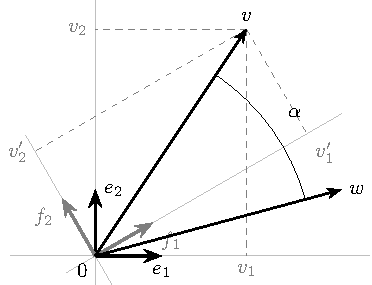
\includegraphics{two_bases.pdf}
    \caption{Two vectors $v$ and $w$ in two orthonormal bases, $\{e_1, e_2\}$ and the rotated basis $\{f_1, f_2\}$. The dashed lines project $v$ onto each basis vector. The components change from basis to basis, whereas the length of $v$ and the angle $\alpha$ do not.}
    \label{fig:bases}
\end{figure}

\paragraph{Orthogonality is defined by the inner product, not by the picture.} A right angle is the usual picture of orthogonality, but the picture already assumes the Euclidean inner product of the drawing plane. Two vectors are orthogonal when $\langle u | v \rangle = 0$, so a basis is orthonormal or skewed only with respect to a chosen inner product. The basis vectors $|g_1\rangle = (1, 0)$ and $|g_2\rangle = (-\tfrac{1}{2}, \tfrac{\sqrt{3}}{2})$, for example, are unit vectors at $120^\circ$ in the drawing plane. The Euclidean inner product of the two basis vectors is
\begin{equation*}
    \langle g_1 | g_2 \rangle = \cos 120^\circ = -\tfrac{1}{2}
\end{equation*}
The inner product is not zero, so the basis is not orthogonal under the Euclidean inner product. Written in its own coordinates, every basis looks like a set of unit columns, so $|g_1\rangle$ and $|g_2\rangle$ become $(1, 0)$ and $(0, 1)$. The sum of products of these columns is zero, but the sum-of-products formula assumes the orthonormality that is being tested, so the argument is circular. The same basis does become orthonormal under a new inner product, defined by $\langle g_i | g_j \rangle' = \delta_{ij}$ and extended linearly. Under the new inner product, however, the Euclidean axes $|\hat x\rangle = (1,0)$ and $|\hat y\rangle = (0,1)$ are no longer orthogonal. The axes expanded in the skewed basis are
\begin{equation*}
    |\hat x\rangle = |g_1\rangle, \qquad
    |\hat y\rangle = \tfrac{1}{\sqrt{3}}\,|g_1\rangle + \tfrac{2}{\sqrt{3}}\,|g_2\rangle
\end{equation*}
and the new inner product of the axes is
\begin{align*}
    \langle \hat x | \hat y \rangle' &= 1 \cdot \tfrac{1}{\sqrt{3}} + 0 \cdot \tfrac{2}{\sqrt{3}} \\
    &= \tfrac{1}{\sqrt{3}} \neq 0
\end{align*}
Each basis is, therefore, orthonormal under the inner product calibrated with that basis, and one inner product cannot make every basis orthonormal at the same time.

\paragraph{A rescaled basis changes the components, not the length.} The basis $|e_i'\rangle = 2|e_i\rangle$ is orthogonal but not normalized, with $\langle e_i' | e_j' \rangle = 4\,\delta_{ij}$. The same vector rewritten in the rescaled basis has half the components:
\begin{equation*}
    |v\rangle = \sum_i v_i\, |e_i\rangle = \sum_i \frac{v_i}{2}\, \bigl(2|e_i\rangle\bigr), \qquad v_i' = \frac{v_i}{2}
\end{equation*}
The squared length, computed with the inner products of the rescaled basis vectors, is unchanged:
\begin{align*}
    \langle v | v \rangle &= \sum_{i,j} v_i'^{*}\, v_j'\, \langle e_i' | e_j' \rangle \\
    &= 4 \sum_i |v_i'|^2 \\
    &= \sum_i |v_i|^2
\end{align*}
The sum of products $\sum_i |v_i'|^2$ would give one quarter of the squared length, because that formula holds only in an orthonormal basis. A rescaled basis and a skewed basis both fail to be orthonormal, the first because the basis vectors are not unit vectors and the second because the basis vectors are not orthogonal. In both cases the ruler fixes the length, and only the components and the formula change. Declaring $2|e_i\rangle$ to have unit length is a different ruler, which halves every length like a change of units.

\paragraph{The orthonormal bases of one inner product are linked by rotations and reflections.} Two orthonormal bases $\{|e_j\rangle\}$ and $\{|f_i\rangle\}$ under the same inner product are linked by a matrix $R$, with $|f_i\rangle = \sum_j R_{ji}\, |e_j\rangle$. The orthonormality of the new basis constrains $R$:
\begin{align*}
    \langle f_i | f_k \rangle &= \sum_{j,l} R_{ji}\, R_{lk}\, \langle e_j | e_l \rangle \\
    &= \sum_{j} R_{ji}\, R_{jk} \\
    &= (R^{T} R)_{ik}
\end{align*}
The condition $\langle f_i | f_k \rangle = \delta_{ik}$ then gives
\begin{equation}
    \boxed{R^{T} R = \mathbb{I}}
\end{equation}
A real matrix with $R^{T} R = \mathbb{I}$ is a rotation or a reflection, as in Fig.~\ref{fig:bases}. For complex coefficients, the transpose becomes the conjugate transpose, and the condition becomes $U^{\dagger} U = \mathbb{I}$ for a \textcolor{blue}{unitary} matrix $U$. Unitary transformations are, therefore, the complex version of rotations and reflections.

\paragraph{Summary of the misconceptions.} Table~\ref{tab:misconceptions} collects the misconceptions corrected in this section.

\begin{table}[h]
    \centering
    \caption{Common misconceptions about vectors, bases and inner products.}
    \label{tab:misconceptions}
    \renewcommand{\arraystretch}{1.3}
    \begin{tabular}{p{0.42\textwidth}p{0.48\textwidth}}
        \toprule
        Misconception & Correction \\
        \midrule
        The component $\langle e_i | v \rangle$ is the projection of $|v\rangle$. & The component is a number. The projection is the vector $|e_i\rangle\langle e_i | v \rangle$. \\
        The basis sets the length of a vector. & The inner product sets the length. Only the components depend on the basis. \\
        $|u|\,|v|\cos\theta$ defines the inner product. & The lengths and the angle are defined by the inner product, so the form is circular. \\
        Orthogonality means a right angle in the picture. & Orthogonality means $\langle u | v \rangle = 0$ under the chosen inner product. \\
        Every basis is orthonormal within itself, because the basis looks like unit columns in its own coordinates. & The sum-of-products formula assumes orthonormality, so the test is circular. \\
        The inner product is defined locally within each basis. & One inner product gives one number. The formulas in the bases are derived from it. \\
        Rescaling the basis by 2 halves the length. & Only the components halve. The formula picks up the factor $\langle e_i' | e_i' \rangle = 4$. \\
        \bottomrule
    \end{tabular}
\end{table}
                      % Section 1: Abstract Linear Space
%% Section 2 of QM.tex (Quantum Mechanics Review). Compile QM.tex, not this file.
%% ============================================================
\section{Quantum Mechanics as an Example}
%% ============================================================

\paragraph{The quantum state is a vector in a Hilbert space.} A quantum state $|\Phi\rangle$ of a system with Hamiltonian $\hat H$ is an abstract \textcolor{blue}{state vector} in a Hilbert space $\mathcal{H}$, so the state obeys every rule in Table~\ref{tab:axioms}. The closure under addition is the superposition principle. The state itself is not measured. Measurements give values of the \textcolor{blue}{observables}, such as momentum, energy and angular momentum, and the state determines the probability of each value. Physics fixes the inner product of $\mathcal{H}$, because the probability $|\langle \Psi | \Phi \rangle|^2$ is measured. A formula that gave a different number in a different basis would, therefore, predict a different experimental result. Quantum mechanics calibrates the ruler with the position basis, $\langle \Psi | \Phi \rangle = \int dx\, \Psi^{*}(x)\, \Phi(x)$. The Born rule makes $|\Phi(x)|^2$ a probability density, so the squared length must be $\int dx\, |\Phi(x)|^2$. A Hermitian Hamiltonian also conserves the total probability, because the time evolution that the Hamiltonian generates is unitary under this inner product.

\paragraph{The wavefunction is the state written in the position basis.} The familiar wavefunction $\Phi(x)$ is not the state itself. The wavefunction is the \textcolor{blue}{position representation} of the state vector, and the other observables, such as momentum, can be calculated from it. Each value $\Phi(x)$ is the component of $|\Phi\rangle$ along the \textcolor{blue}{position eigenstate} $|x\rangle$:
\begin{equation}
    \boxed{\Phi(x) = \langle x | \Phi \rangle}
\end{equation}
The wavefunction is, therefore, a \textcolor{blue}{probability amplitude}. The value $\Phi(x)$ is a complex number, and the squared modulus $|\Phi(x)|^2$ is the probability density. The amplitude is the square root of the probability density, up to a phase $\theta(x)$:
\begin{equation*}
    \Phi(x) = \sqrt{|\Phi(x)|^2}\; e^{i\theta(x)}
\end{equation*}

\paragraph{The position eigenbasis is a continuous orthonormal basis.} The wavefunction is an infinite array with one complex number for each position $x$, with the position $x$ in the role of the index $i$ in Section~1. The sum over $i$ becomes an integral, and the Kronecker delta becomes the Dirac delta, $\langle x | x' \rangle = \delta(x - x')$. The completeness relation of the position eigenbasis is
\begin{equation*}
    \int dx'\, |x'\rangle\langle x'| = \mathbb{I}
\end{equation*}
Inserting the completeness relation in front of $|\Phi\rangle$ gives
\begin{equation*}
    |\Phi\rangle = \int dx'\, |x'\rangle\langle x' | \Phi \rangle
\end{equation*}
\begin{equation}
    \boxed{|\Phi\rangle = \int dx'\, \Phi(x')\, |x'\rangle}
\end{equation}
The primed variable $x'$ is a placeholder that runs over every position eigenstate, like the summation index $i$, and renaming $x'$ does not change the expansion. The unprimed variable $x$ is the single position at which the wavefunction is evaluated, like the fixed index $j$. The projection of the expansion back onto $\langle x|$, therefore, recovers one entry of the array:
\begin{align*}
    \langle x | \Phi \rangle &= \int dx'\, \Phi(x')\, \langle x | x' \rangle \\
    &= \int dx'\, \Phi(x')\, \delta(x - x') \\
    &= \Phi(x)
\end{align*}
The delta function selects the entry at $x' = x$ in the same way that the Kronecker delta $\delta_{ji}$ selects the component $v_j$. The position eigenstates are not normalizable, because $\langle x | x \rangle = \delta(0)$ diverges. Strictly, $|x\rangle$ lies outside $\mathcal{H}$, and the rigorous framework is the \textcolor{blue}{rigged Hilbert space}. The position eigenstates are still used as a basis, because every physical state is a normalizable superposition of them.

\paragraph{Discretizing the wavefunction turns the integral into a sum over array entries.} The array picture becomes concrete when the position axis is cut into points $x_i = i\,\Delta x$ with a small spacing $\Delta x$. Figure~\ref{fig:array} uses the wavefunction $\Phi(x) = \sqrt{2/\pi}\,\sin x$ on the interval $0 \leq x \leq \pi$, which is the ground state of an infinite square well of width $\pi$. Each point $x_i$ stores one number $\Phi(x_i)$, and the list of these numbers is a column vector with $N$ entries. The integral over $x'$ in the expansion of $|\Phi\rangle$ is the limit of a sum over these entries:
\begin{equation*}
    |\Phi\rangle = \int dx'\, \Phi(x')\, |x'\rangle = \lim_{\Delta x \to 0}\, \sum_{i=1}^{N} \Delta x\, \Phi(x_i)\, |x_i\rangle
\end{equation*}
The number of entries $N = \pi/\Delta x$ grows without limit as $\Delta x \to 0$. The finite column vector, therefore, becomes the continuous function $\Phi(x)$ with one entry for every real number $x$.

\begin{figure}[h]
    \centering
    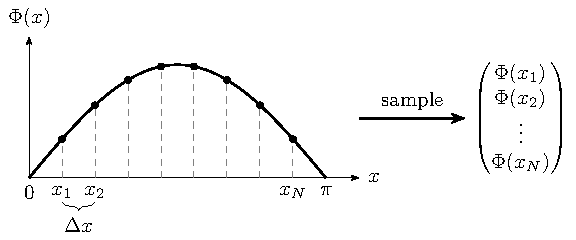
\includegraphics{wavefunction_array.pdf}
    \caption{Wavefunction $\Phi(x) = \sqrt{2/\pi}\,\sin x$ sampled at $N$ points with spacing $\Delta x$. The sampled values form a column vector with $N$ entries. The column vector becomes the continuous function for $\Delta x \to 0$ and $N \to \infty$.}
    \label{fig:array}
\end{figure}

\paragraph{A function is also an abstract vector.} The whole function $\Phi$, rather than a single value $\Phi(x)$, is itself a vector for the same reason as $|\Phi\rangle$. The \textcolor{blue}{square-integrable functions}, with $\int |\Phi(x)|^2\, dx$ finite, form the vector space $L^2$. The sum of two square-integrable functions is square-integrable, a complex multiple of a square-integrable function is square-integrable, and the zero function is the zero vector. The functions, therefore, obey every rule in Table~\ref{tab:axioms}. The inner product in the position basis follows from the completeness relation:
\begin{align*}
    \langle \Psi | \Phi \rangle &= \int dx\, \langle \Psi | x \rangle \langle x | \Phi \rangle \\
    &= \int dx\, \langle x | \Psi \rangle^* \langle x | \Phi \rangle
\end{align*}
\begin{equation}
    \boxed{\langle \Psi | \Phi \rangle = \int dx\, \Psi^*(x)\, \Phi(x)}
\end{equation}
The integral is the continuous version of the sum of products in Section~1, so the integral is the formula of the inner product in the position basis rather than the definition of the inner product. The squared length $\langle \Phi | \Phi \rangle = \int dx\, |\Phi(x)|^2$ is the special case of a state with itself. The map from $|\Phi\rangle$ to $\Phi(x)$ keeps sums, complex multiples and inner products unchanged. The Hilbert space $\mathcal{H}$ and the function space $L^2$ are, therefore, two descriptions of the same vectors. The state vector is the basis-free description, and the wavefunction is the description in the position basis.

\paragraph{The momentum eigenbasis gives another representation of the same state.} The state vector can also be expanded in the \textcolor{blue}{momentum eigenbasis}, in the same way as in the position eigenbasis. \textcolor{red}{The momentum representation is written as $\tilde{\Phi}(p)$, with a tilde, to distinguish it from the position representation $\Phi(x)$.} Each value $\tilde{\Phi}(p)$ is the component of $|\Phi\rangle$ along the momentum eigenstate $|p\rangle$:
\begin{equation}
    \boxed{\tilde{\Phi}(p) = \langle p | \Phi \rangle}
\end{equation}
The position and momentum representations are two lists of components for the same state $|\Phi\rangle$, like the two lists $(v_1, v_2)$ and $(v_1', v_2')$ in Fig.~\ref{fig:bases}.

\paragraph{The position and momentum eigenbases are linked by a unitary transformation.} The position and momentum eigenstates are both orthonormal under the same inner product, with $\langle x | x' \rangle = \delta(x - x')$ and $\langle p | p' \rangle = \delta(p - p')$. The change of basis is a matrix with continuous indices, $U(x, p) = \langle x | p \rangle$. The momentum operator acts as $-i\hbar\, d/dx$ in the position representation, so the eigenvalue equation $\hat p |p\rangle = p |p\rangle$ projected onto $\langle x|$ is a differential equation:
\begin{align*}
    \langle x | \hat p | p \rangle &= -i\hbar \frac{d}{dx} \langle x | p \rangle \\
    &= p\, \langle x | p \rangle
\end{align*}
The solution is a plane wave, $\langle x | p \rangle = C\, e^{ipx/\hbar}$, with a constant $C$. The normalization $\langle p | p' \rangle = \delta(p - p')$ fixes $C$, with the completeness relation of the position eigenbasis and $\int dx\, e^{ikx} = 2\pi\, \delta(k)$:
\begin{align*}
    \langle p | p' \rangle &= \int dx\, \langle p | x \rangle \langle x | p' \rangle \\
    &= |C|^2 \int dx\, e^{i(p' - p)x/\hbar} \\
    &= |C|^2\, 2\pi\hbar\, \delta(p - p')
\end{align*}
The choice of a real, positive $C = 1/\sqrt{2\pi\hbar}$ gives
\begin{equation}
    \boxed{\langle x | p \rangle = \frac{1}{\sqrt{2\pi\hbar}}\, e^{ipx/\hbar}}
\end{equation}
The same calculation is the unitarity condition $U^{\dagger} U = \mathbb{I}$ written with continuous indices. The orthonormality of the momentum eigenbasis is, therefore, not automatic. A momentum formula without the factor $C$ would be off by $2\pi\hbar$ and would describe a different inner product. The momentum representation then follows from the position representation by the completeness relation:
\begin{align*}
    \tilde{\Phi}(p) &= \int dx\, \langle p | x \rangle \langle x | \Phi \rangle \\
    &= \int dx\, \langle x | p \rangle^{*}\, \Phi(x)
\end{align*}
\begin{equation}
    \boxed{\tilde{\Phi}(p) = \frac{1}{\sqrt{2\pi\hbar}} \int dx\, e^{-ipx/\hbar}\, \Phi(x)}
\end{equation}
The change from the position to the momentum representation is, therefore, a \textcolor{blue}{Fourier transform}. The reverse change uses the completeness relation of the momentum eigenbasis, $\int dp\, |p\rangle\langle p| = \mathbb{I}$:
\begin{align*}
    \Phi(x) &= \int dp\, \langle x | p \rangle \langle p | \Phi \rangle \\
    &= \frac{1}{\sqrt{2\pi\hbar}} \int dp\, e^{ipx/\hbar}\, \tilde{\Phi}(p)
\end{align*}
The unitary change of basis keeps the inner product unchanged, so the overlap of two states is the same in both representations:
\begin{align*}
    \langle \Psi | \Phi \rangle &= \int dp\, \langle \Psi | p \rangle \langle p | \Phi \rangle \\
    &= \int dp\, \tilde{\Psi}^{*}(p)\, \tilde{\Phi}(p) \\
    &= \int dx\, \Psi^{*}(x)\, \Phi(x)
\end{align*}
Table~\ref{tab:inner} collects the formulas of the inner product in the position basis, the momentum basis and a discrete orthonormal basis $\{|n\rangle\}$, with the components $c_n = \langle n | \Psi \rangle$ and $d_n = \langle n | \Phi \rangle$. Every momentum eigenstate overlaps every position eigenstate with the same magnitude, $|\langle x | p \rangle| = 1/\sqrt{2\pi\hbar}$. The two bases are, therefore, as far from aligned as possible, and a state that is sharp in one representation is spread over the whole of the other.

\begin{table}[h]
    \centering
    \caption{Formulas of the inner product $\langle \Psi | \Phi \rangle$ in three orthonormal bases.}
    \label{tab:inner}
    \renewcommand{\arraystretch}{1.5}
    \begin{tabular}{lll}
        \toprule
        Basis & Completeness relation & Inner product $\langle \Psi | \Phi \rangle$ \\
        \midrule
        Position $\{|x\rangle\}$ & $\int dx\, |x\rangle\langle x| = \mathbb{I}$ & $\int dx\, \Psi^{*}(x)\, \Phi(x)$ \\
        Momentum $\{|p\rangle\}$ & $\int dp\, |p\rangle\langle p| = \mathbb{I}$ & $\int dp\, \tilde{\Psi}^{*}(p)\, \tilde{\Phi}(p)$ \\
        Discrete $\{|n\rangle\}$ & $\sum_n |n\rangle\langle n| = \mathbb{I}$ & $\sum_n c_n^{*}\, d_n$ \\
        \bottomrule
    \end{tabular}
\end{table}
                      % Section 2: Quantum Mechanics as an Example

\end{document}
